\documentclass[border=6pt]{standalone}
% Shared preamble for web figures.  Each figure is a standalone .tex that
% \input's this file; scripts/make-figures.sh turns it into an SVG.
% Handouts pull the same file with \fig{Unit_X/<name>}.
\usepackage[T1]{fontenc}
\usepackage{helvet}
\renewcommand{\familydefault}{\sfdefault}
\renewcommand{\ttdefault}{pcr}  % Courier: a real Type 1 typewriter font
\usepackage{amsmath}
\usepackage{tikz}
\usetikzlibrary{arrows.meta,positioning,calc,shapes.symbols,shapes.geometric}

% Who makes the rules is the point of most diagrams in this book, so the
% colors mean the same thing everywhere: blue is a person, orange is the
% computer, green is an answer, pink is the human brain.
\definecolor{person}{HTML}{2C6FAE}
\definecolor{machine}{HTML}{D35400}
\definecolor{result}{HTML}{1E8449}
\definecolor{brainpink}{HTML}{C2185B}
\definecolor{ink}{HTML}{2C3E50}

\tikzset{
  doodle/.style={line width=1.5pt, line cap=round, line join=round, draw=ink},
  box/.style={draw, rounded corners=5pt, line width=1.1pt, align=center,
              inner sep=7pt, minimum height=1.0cm, font=\small},
  personbox/.style={box, draw=person, fill=person!10},
  machinebox/.style={box, draw=machine, fill=machine!10},
  resultbox/.style={box, draw=result, fill=result!10},
  plainbox/.style={box, draw=ink!70, fill=ink!4},
  flow/.style={-{Stealth[length=8pt]}, line width=1.4pt, draw=ink},
}

% A person (blue) and a robot head (orange) as small icons.
% \personicon{x}{y}{scale}   \roboticon{x}{y}{scale}
\newcommand{\personicon}[3]{%
  \begin{scope}[shift={(#1,#2)}, scale=#3]
    \fill[person] (0,0.62) circle (0.28);
    \fill[person, rounded corners=6pt] (-0.42,-0.55) rectangle (0.42,0.28);
  \end{scope}}
\newcommand{\roboticon}[3]{%
  \begin{scope}[shift={(#1,#2)}, scale=#3]
    \draw[machine, line width=1.2pt] (0,0.5) -- (0,0.72);
    \fill[machine] (0,0.78) circle (0.08);
    \draw[machine, line width=1.4pt, fill=machine!12, rounded corners=4pt] (-0.5,-0.45) rectangle (0.5,0.5);
    \fill[ink] (-0.2,0.12) circle (0.08);
    \fill[ink] (0.2,0.12) circle (0.08);
    \draw[ink, line width=1pt] (-0.22,-0.22) -- (0.22,-0.22);
  \end{scope}}

\begin{document}
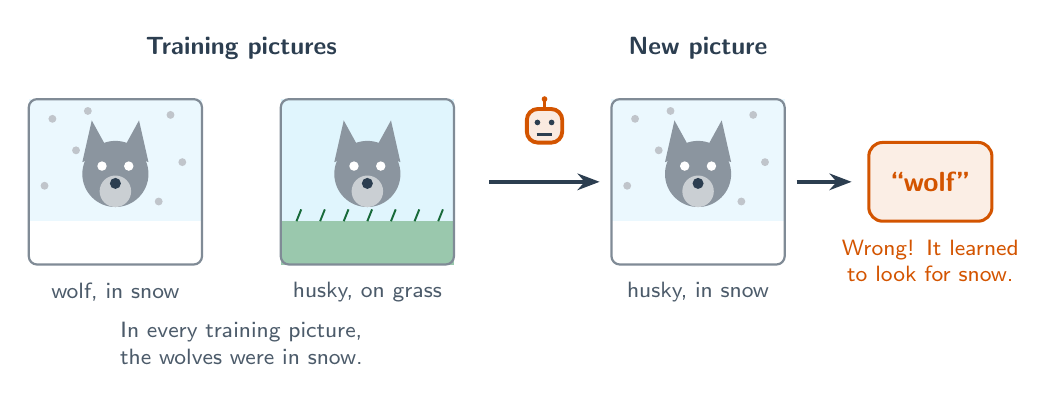
\begin{tikzpicture}[
  ttl/.style={font=\small\bfseries, text=ink, align=center},
  sub/.style={font=\footnotesize, text=ink!85, align=center},
]
% The "wolf detector" that learned snow (Ribeiro, Singh and Guestrin, 2016).
% \scene{x}{snow or grass}{label}
\newcommand{\head}[2]{% x, y: a simple dog/wolf head
  \begin{scope}[shift={(#1,#2)}]
    \fill[ink!55] (-0.42,0.25) -- (-0.30,0.78) -- (-0.08,0.38) -- cycle;
    \fill[ink!55] (0.42,0.25) -- (0.30,0.78) -- (0.08,0.38) -- cycle;
    \fill[ink!55] (0,0.1) circle (0.42);
    \fill[ink!25] (0,-0.12) ellipse (0.2 and 0.2);
    \fill[ink] (0,-0.02) circle (0.07);
    \fill[white] (-0.17,0.2) circle (0.06); \fill[white] (0.17,0.2) circle (0.06);
  \end{scope}}
\newcommand{\snow}[1]{% x: snowy scene
  \fill[cyan!8] (#1-1.1,-1.0) rectangle (#1+1.1,1.1);
  \fill[white] (#1-1.1,-1.0) rectangle (#1+1.1,-0.45);
  \foreach \a/\b in {-0.8/0.85,-0.5/0.45,0.7/0.9,0.85/0.3,-0.9/0.0,0.55/-0.2,-0.35/0.95} \fill[ink!30] (#1+\a,\b) circle (0.05);
  \draw[ink!60, line width=0.8pt, rounded corners=3pt] (#1-1.1,-1.0) rectangle (#1+1.1,1.1);}
\newcommand{\grass}[1]{% x: grassy scene
  \fill[cyan!12] (#1-1.1,-1.0) rectangle (#1+1.1,1.1);
  \fill[result!45] (#1-1.1,-1.0) rectangle (#1+1.1,-0.45);
  \foreach \a in {-0.9,-0.6,...,0.9} \draw[result!80!black, line width=0.7pt] (#1+\a,-0.45) -- (#1+\a+0.06,-0.3);
  \draw[ink!60, line width=0.8pt, rounded corners=3pt] (#1-1.1,-1.0) rectangle (#1+1.1,1.1);}

\node[ttl] at (1.6,1.75) {Training pictures};
\snow{0}  \head{0}{0.05}  \node[sub] at (0,-1.35) {wolf, in snow};
\grass{3.2} \head{3.2}{0.05} \node[sub] at (3.2,-1.35) {husky, on grass};
\node[sub, text width=5cm] at (1.6,-2.0) {In every training picture, the wolves were in snow.};

\draw[flow] (4.75,0.05) -- (6.15,0.05);
\roboticon{5.45}{0.75}{0.45}

\node[ttl] at (7.4,1.75) {New picture};
\snow{7.4} \head{7.4}{0.05} \node[sub] at (7.4,-1.35) {husky, in snow};
\draw[flow] (8.65,0.05) -- (9.35,0.05);
\node[box, fill=machine!10, draw=machine, font=\bfseries, text=machine] at (10.35,0.05) {``wolf''};
\node[sub, text=machine, text width=2.4cm] at (10.35,-0.95) {Wrong! It learned to look for snow.};
\end{tikzpicture}
\end{document}
